\documentclass{article}
\usepackage{graphicx} % Required for inserting images
\usepackage{geometry}
\usepackage{textcomp}
\usepackage{graphicx}
 \geometry{
 a4paper,
 total={170mm,257mm},
 left=20mm,
 top=20mm,
 }
\title{\textbf{AA 260 Lab 5}}
\author{Hugh Carbrey, Matthew Idso, Jeffery Zhang}
\date{July 26th, 2023}

\begin{document}

\maketitle
\section{Problem}
You decide that your house needs a new water heater. Your previous water heater was electric,
had an efficiency of 92\%, and cost \$423 a year to operate when electricity cost \$0.13/kWh. One option is to replace it with a the same unit. The other option is to buy a heat pump powered
water heater that has a COP of 3.3, but costs about \$1000 more (for both the actual unit and
installation). \textbf{Determine how many years it will take for the heat pump water heater to pay for its cost differential from the energy it saves.} \\*[10pt]
Investigate the effect of the COP on the payback period for the heat pump option. \textbf{Plot the payback period vs COP for values between 2 and 5, and discuss the results.}

\section{Assumptions}
\begin{itemize}
    \item All relevant quantities are steady across any given year (which allows for interpolation and averaging)
    \item Both heaters produce the exact same amount of heat within a given year.
    \item Prices remain constant within a given year.
    \item There is no loss in efficiency or performance in either heat pump over the course of measurement.
    \item Environmental temperature remains the same over the course of measurement.
    \item We want a constant water temperature.
\end{itemize}
\section{Procedure}
\subsection{Part 1}
First, we find the amount of heat transferred to the water in a year. This is found by multiplying the efficiency of the old heat engine by the electricity power input.
\begin{center}
    \(\displaystyle \frac{\$423}{year}\cdot \frac{1 \: kWh}{\$0.13} = 3254\:\frac{kWh}{year}\)\\*[10pt]
    \(\displaystyle 3254\:\frac{kWh}{year} \cdot 0.92 = 2994\:\frac{kWh}{year}\)\\*[10pt]
    \(\displaystyle 2994\:\frac{kWh}{year}\cdot \frac{3600\:kJ}{1 kWh}\cdot \frac{1\:GJ}{10\cdot 10^6 \: kJ} = 10.8 \:\frac{GJ}{year}\)
\end{center}
Next, we use the following equation to relate the amount of heat transferred to the new \(COP_H\) value.
\begin{center}
    \(\displaystyle COP_{H, new} = \frac{Q_H}{W_{in}}\)\\*[10pt]
    \(\displaystyle W_{in} = \frac{Q_H}{COP_{H, new}}\)\\*[10pt]
    \(\displaystyle W_{in} = \frac{10.8\:\frac{GJ}{year}}{3.3} = 3.27\:\frac{GJ}{year}\)
\end{center}
\clearpage \noindent
Therefore,
\begin{center}
    \(\displaystyle 3.27\:\frac{GJ}{year}\cdot \frac{10\cdot 10^6 \: kJ}{1\:GJ} \cdot \frac{1 kWh}{3600 kJ} = 907 \:\frac{kWh}{year}\)
\end{center}
Finally,
\begin{center}
    \(\displaystyle 3254 \:\frac{kWh}{year} - 907 \:\frac{kWh}{year} = 2347 \:\frac{kWh}{year}\) saved \\*[10pt]
    \(\displaystyle 2347\:\frac{kWh}{year}\cdot \frac{\$0.13}{kWh} = \$305.11\) per year \\*[10pt]
    \(\displaystyle \frac{\$1000}{\frac{\$305.11}{year}} =\:\) \textbf{3.28 years}
\end{center}
\clearpage \noindent
\begin{figure}
    \centering
    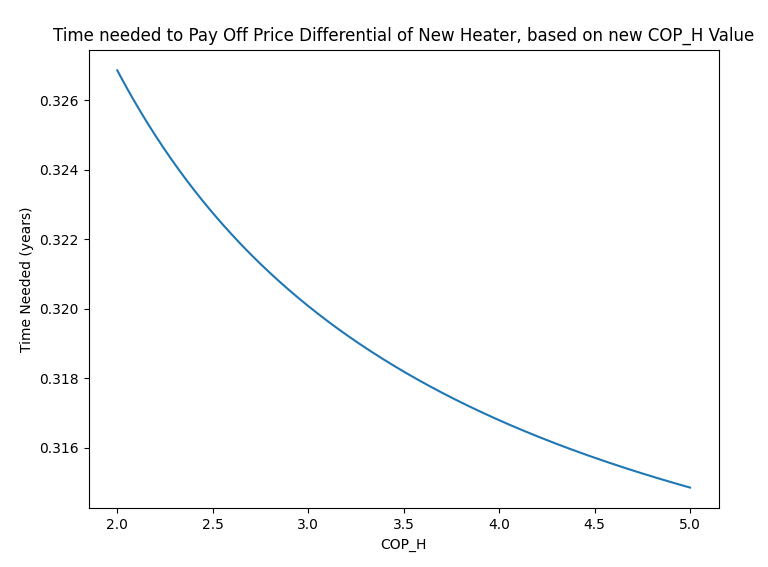
\includegraphics[width = \textwidth]{figs/lol.png}
    \caption{Our graph (Made using Python)}
    \label{fig:enter-label}
\end{figure}
\subsection{Part 2}
This graph makes both intuitive and mathematical sense. As the coefficient of performance increases, the rate at which the price differential is paid off increases. Therefore, the time interval during which the differential must be paid off becomes shorter and shorter. Mathematically, per the equation:
\begin{center}
    \(\displaystyle COP_{H, new} = \frac{Q_H}{W_{in}}\)\\*[10pt]
\end{center}
Since we know the goal \(Q_H\) remains constant, the coefficient of performance for the heater is inversely proportional to the amount of electric power needed (and thus, money that needs to be paid). In other words, as the coefficient of performance goes up, less electric power is necessitated, saving money.
\end{document}
